
\chapter{Research design}
This chapter contains the information on how the research will be conducted.

\section{Research objective}

\subsection{The problem}
\label{sec:TheProblem}

Right now EFFE is developing an application for employment agencies in which those employment agencies can schedule their employees automatically. The current application is really basic and there are requests from potential clients to implement certain features. The decision has been made to add something to the business model called building blocks.

\largequote{Building blocks are interchangeable implementations of business logic that can be reused as efficient as possible}

EFFE is looking how to implement the building blocks in such a manner where scalability and maintainability are the focus.

\subsection{Objective}
The objective is to create a recommendation for an infrastructure on how to create and maintain that infrastructure. Where the focus lays on interchangeability and scalability of the different functionalities.

\begin{tabularx}{\linewidth}{|>{\hsize=.3\hsize}X|>{\hsize=.7\hsize}X|}
	\hline
	Stakeholder &
	Interest to the objective
	\\
	\hline
	EFFE &
	The obvious stakeholder is EFFE. EFFE will enhance its business model. But not only that. EFFE will also create a better infrastructure which means that she can implement functionalities faster and cater more to the clients’ need.
	\\
	\hline
	Client &
	The client is also the one interested in this process. They are probably not interested into what happens behind the scenes, but they are interested in the possibilities it adds for them to EFFE’s application
	\\
	\hline
\end{tabularx}

\section{Research framework}

\subsection{Objects}
This chapter describes who/what the objects are for this research and why.

\subsubsection{Backend architecture}
Arguably the most important object is the backend architecture. There is already a lot of research available regarding backend architecture. The backend is also the place where the business logic will be expressed. The backend connects to the database and thus needs a lot of attention when creating this section of the application.

\subsubsection{Frontend architecture}
The second object, frontend architecture, is a lesser known subject when looking at modularity of the actual system. Most of the big companies have a single frontend application per platform.

\subsubsection{Deployment lane}
\label{sec:DeploymentLane}
The backend and the frontend are the software side of the equation but the hardware is also important. Where does the software run? How does it run? The deployment lane is the section that pieces it all together. This object creates the hardware or virtual hardware. Sets this hardware up so it can then proceed to deploy the frontend and backend on the just created hardware. This process is very important and EFFE is not the first company wanting to adopt this. Which means there is already a lot of research in this area.

\subsubsection{Software architect}
\label{sec:SoftwareArchitect}
The last object to be researched is the software architect. The software architects job is to design how the system will be build. This can be small scale like a naming convention but also bigger scale like layered architecture or modular architecture. Even the programming language can be decided by a software architect because each language has its own pros and cons.

\subsection{Research perspective}
The research perspective is straight forward. Because I am one of the founders of EFFE and I am also doing this research in name of EFFE it has my best interest to approach this research from the side of EFFE. This means that I will put more emphasis on sustainability than for example on the performance. Because for now performance can be dealt with later but if you want something to be sustainable you have to think about it from the ground up. Otherwise you will need to rewrite the whole architecture.

\subsection{Research sources}
This section will describe which sources will be used when evaluating the research objects. This will not include everything but a broad spectrum of the sources that may be used in the research:

\begin{itemize}
	\item \textbf{Modular architecture books: }In the end everything I need to know all comes down to modular programming. Modular programming is a very broad term and it is important to find how someone else may look at this term.

	\item \textbf{Implementations of modular programming: }Theory is one side of the coin. Everything can work perfectly in theory but when implementing the theoretic side you will find problems you haven't thought of before.

	\item \textbf{Critique from outside: }It is known that software architecture is an opinion based subject. This is because especially this area of software is fairly young. Software architecture did not have a lot of time to develop itself as far as some other aspects of software engineering such as operating systems. Because software architecture is young there are a lot of people voicing their opinions and it is important to look at the criticism on some of the architectures.

	\item \textbf{Researches on deployment of architecture: }I will be researching more than one architecture. Each architecture has its own development environment and deployment environment. The architecture of the servers on which the program runs is important but that will be heavily influenced by the architecture of the software. Nevertheless should it be researched separately from the software architecture
\end{itemize}

\subsection{Evaluation criteria}
These are the criteria or leading questions that will be asked to research objects. Note: not all evaluation criteria apply to all research objects:

\begin{itemize}
	\item \textbf{What is the biggest pitfall when implementing a new architecture: }As mentioned in \fullref{sec:SoftwareArchitect} the software architect makes the choices arount the architecture. So it is important to look at what can go wrong when implementing a new architecture. What are the common pitfalls they have experienced when implementing a new architecture.

	\item \textbf{What are the most used architectures in this area: }There is always a reason why one architecture is very common and the other one isn't. In the research the reasoning will be extracted and reflected on.

	\item \textbf{What are the most upcoming architectures that are focused on modularity: }Again the whole research is based on the building blocks. These modular functionalities that can be designed via a common interface. Which architecture has which solution for this?

	\item \textbf{Which programming languages has the best attributes to complement the modularity: }Some languages are written purely for scripting or some are written to be focused on implementing algorithms more easily. Each programming language has its attributes and which of these attributes are most defining and important to a modular system.

	\item \textbf{Which quality attributes are deemed most important to EFFE?: }The quality attributes from ISO 205010 \cite{iso25010} are the backbone of an the architecture. In the research will describe which are most important to EFFE. It is than important to reflect the quality attributes EFFE chose on the architectures.
\end{itemize}

\subsection{Research framework}

\begin{figure}[H]
	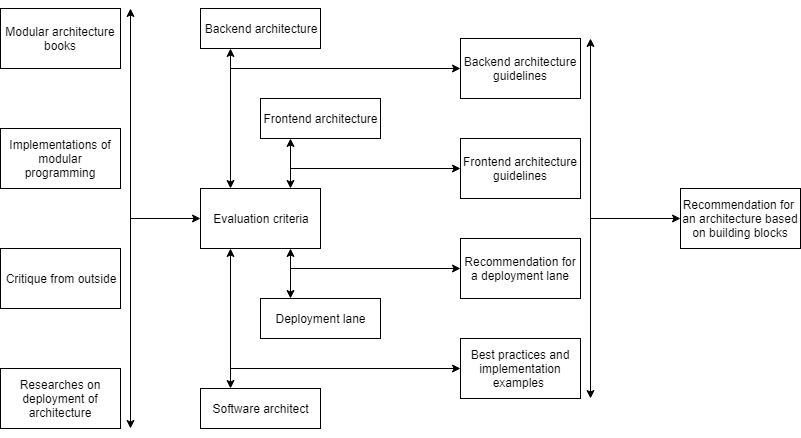
\includegraphics[width=\linewidth]{research_framework.png}
	\caption{Research framework}
\end{figure}

\subsection{Expected Results}

The results will be the guidelines on which the practical part of this research will be based.

\begin{itemize}
	\item \textbf{Backend architecture guidelines: } These are the guidelines on which the backend architecture will be based on. These guidelines will indicate why I choose for a certain approach and what the specific approach is.

	\item \textbf{Frontend architecture guidelines: } These are the guidelines for the frontend. Such as the backend guidelines these guidelines will also contain the reasoning for a certain guideline.

	\item \textbf{Recommendation for a deployment lane: } As mentioned in \fullref{sec:DeploymentLane} the deployment lane can impact the backend architecture and vise versa. This recommendation will be implemented and should thus work perfectly with the backend and frontend.

	\item \textbf{Best practices and implementation examples: } What the software architect experiences and what can go wrong is important to then again pass to the evaluation criteria.
\end{itemize}

\section{Research Questions}
Note: question 2 and 3 will be handled separately for both backend and frontend.

\subsection{Main question}
From this the main question can be derived:

\largequote{What is the best way to transform a monolith into a modular architecture, where the services are interchangeable from each other}

\subsection{Question 1}
\label{sec:Question1}
The first question that will be asked is what is the purpose of this question. The first question is about software architecture. How does a software architect create a software architecture. The model can be found in the appendix under Creating a software architecture.

The thicker red lines show the parts of the model I want to explore in the question. Thus the question is:

\largequote{What was the thought process behind choosing certain implementations for the quality attributes of a software architecture?}

This question will explore how a software architect chooses the architecture. This will give more insights into what they consider when choosing an implementations so that their rational can be extracted and taken into consideration.

These are some of the sub questions that will be handled based on this central question
\begin{itemize}
	\item Which techniques are used when mapping the priority and the drawbacks in order to make a decision?
	\item How does the priority of a quality attribute influence the end result or software architecture?
	\item How does the software architect combine the priority, drawbacks and possible implementations to a software architecture?
\end{itemize}

\subsection{Question 2}
\largequote{Which software architectures that focus on modularity are available?}

This question focuses on the architecture that are available. The knowledge of how a software architect chooses the architecture is answered in the previous question \fullref{sec:Question1}. In this question there will be a search on the architectures that are available and how they came to be.. Because of the new perspective gotten from the previous question there can be a more nuanced look at the architecture.

Here are some of the sub questions:
\begin{itemize}
	\item Which are the upsides and downsides of each architecture?
	\item On what level is the documentation and research surrounding the architecture?
	\item Which architecture implements the quality attributes I deemed important best?
\end{itemize}

\subsection{Question 3}
\largequote{Which implementations are there of the solutions provided for modular architecture?}

The solutions or architectures provided from question 2 will have implementations or frameworks. It is important to see which implementation implements a certain choice of the architecture in what way. Other questions that will be answered are:
\begin{itemize}
	\item How mature is the architecture in contrast to the implementations?
	\item How does the language chosen in the implementation reflect to the architecture?
	\item On what level does the framework compromise which is not reflected in the architecture?
	\item How is the community of this implementation?
\end{itemize}

\subsection{Question 4}

\largequote{What are the key elements of in which a software architecture will influence the deployment lane?}

This question hints at the relation between a software architecture and the deployment lane. Right now there is a limited view on how the deployment lane should be and how it can be. In order for the practical research to work there needs to be an answer to these questions:
\begin{itemize}
	\item Which infrastructure fits best with my chosen architecture?
	\item What are the costs of different infrastructures?
	\item How does the infrastructure implement our quality attributes
\end{itemize}
